\documentclass{article}
\usepackage[legalpaper, landscape, margin=1in]{geometry}
\usepackage{amsmath}
\usepackage{scalerel}
\usepackage{graphicx}


%\[\frac{a}{b}\ \myfrac{a}{b}\ \myfrac[1pt]{a}{b}\ \myfrac[3pt]{a}{b}\ \myfrac[3pt]{a}{b}\]

\RequirePackage{fix-cm} % arbitrary font scaling
\makeatletter
\renewcommand*\env@matrix[1][*\c@MaxMatrixCols c]{%
  \hskip -\arraycolsep
  \let\@ifnextchar\new@ifnextchar
  \array{#1}}
\makeatother
\newcommand{\RomCap}[1]
    {\MakeUppercase{\scaleto{\romannumeral #1}{3.5pt}}}
\DeclareMathSizes{10}{10}{8}{5}
\newcommand{\myfrac}[3][0pt]{\genfrac{}{}{}{}{\raisebox{#1}{$#2$}}{\raisebox{-#1}{$#3$}}}
\begin{document}
\section{Governing integral equations for two-region continuum electrostatics problem}
\subsection{Problem schematic}

\begin{center}
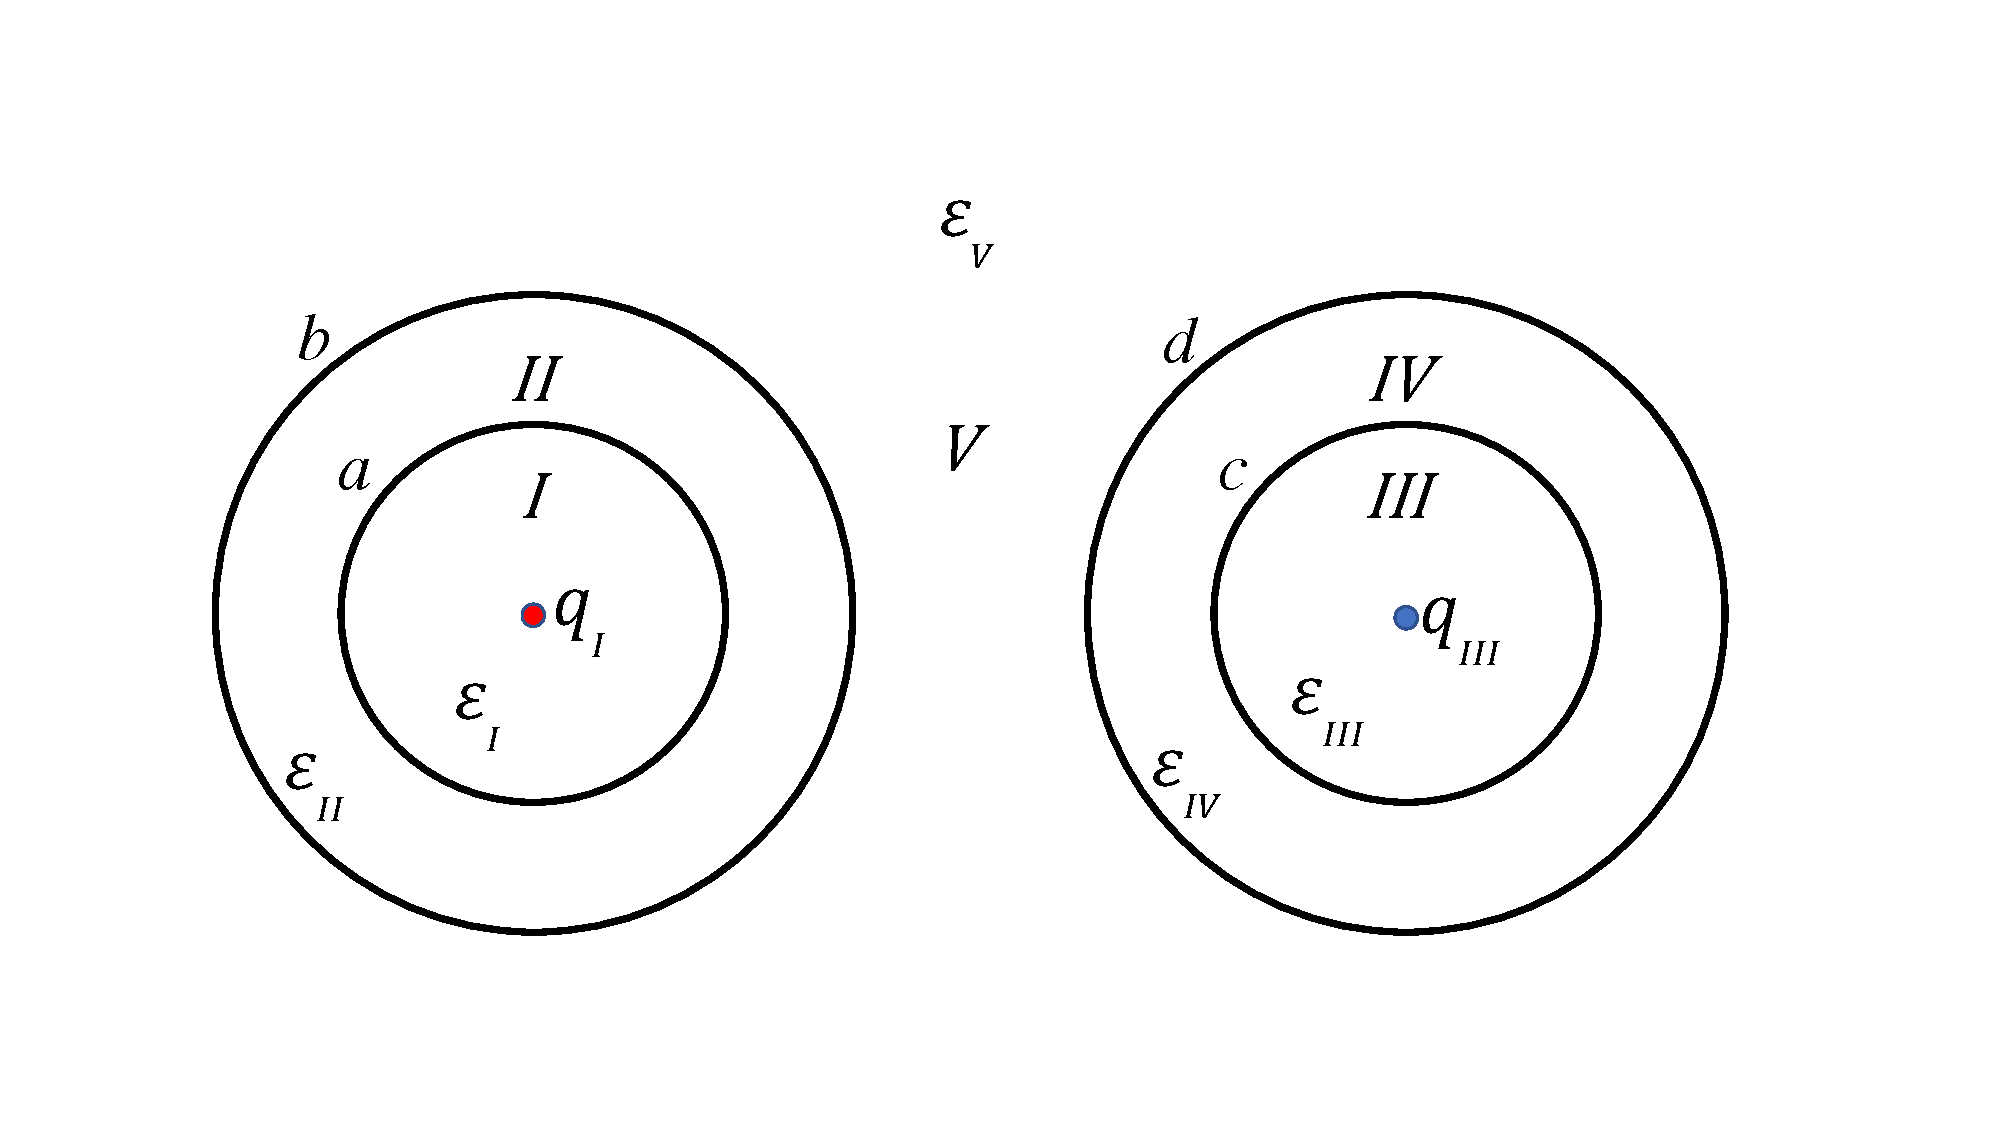
\includegraphics[width=18cm, height=10cm]{schematic.pdf}
\end{center}

\subsection{Two-region intergal equation using classical continuum theory}


    \begin{equation}
    	\begin{bmatrix}[cccc|cccc]
    		\\
            \iffalse
	     	Row 1 : A_{11} & A_{12} &
			\fi

            \frac{1}{2}I+K^{a}_{\RomCap{1},a} & -V^{a}_{\RomCap{1},a} & 	

            \iffalse
	     	A_{31} & A_{41} & A_{51} & A_{61} & A_{71} & A_{81} \\
			\fi

             &  &  &  &  &  \\ 
             &  &  &  &  &  &  & \\
	     	
	     	\iffalse
	     	Row 2 : A_{21} &
			\fi
			
			\frac{1}{2}I-K^{a}_{\RomCap{2},a} & 	
			
			\iffalse
	     	A_{22} &
			\fi
	     	
	     	\big(\myfrac[3pt]{\epsilon_{_\RomCap{1}}}{\epsilon_{_\RomCap{2}}}\big)V^{a}_{\RomCap{2},a} &
	     	
	     	\iffalse
	     	A_{23} & A_{24} &
			\fi

			K^{a}_{\RomCap{2},b} & -V^{a}_{\RomCap{2},b} & 

	     	\iffalse
	     	A_{25} & A_{26} & A_{27} & A_{28} \\
	     	\fi
			
	     	 &	 &  &  \\ 
             &  &  &  &  &  &  & \\
	     	\iffalse
	     	Row 3 : A_{31} &
			\fi
			
			-K^{b}_{\RomCap{2},a} & 	
			
			\iffalse
	     	A_{32} &
			\fi
	     	
	     	\big(\myfrac[3pt]{\epsilon_{_\RomCap{1}}}{\epsilon_{_\RomCap{2}}}\big)V^{b}_{\RomCap{2},a} &
	     	
	     	\iffalse
	     	A_{33} & A_{34} &
			\fi

			\frac{1}{2}I+K^{b}_{\RomCap{2},b} & -V^{b}_{\RomCap{2},b} &

	     	\iffalse
	     	A_{35} & A_{36} & A_{37} & A_{38} \\
	     	\fi
			
	     	 &	 &  & \\ 
             &  &  &  &  &  &  & \\
	     	\iffalse
	     	Row 4 : A_{41} & A_{42} &
			\fi
			
			 &  & 	
			
			\iffalse
	     	A_{43} &
			\fi

			\frac{1}{2}I-K^{b}_{\RomCap{5},b} & 

			\iffalse
	     	A_{44} &
			\fi

			\big(\myfrac[3pt]{\epsilon_{_\RomCap{2}}}{\epsilon_{_\RomCap{5}}}\big)V^{b}_{\RomCap{5},b} &

	     	\iffalse
	     	A_{45} & A_{46} & 
	     	\fi
			
	     	 &	 &

	     	\iffalse
	     	A_{47} & 
	     	\fi
			
	     	-K^{b}_{\RomCap{5},d} &

			\iffalse
	     	A_{48} \\
			\fi

			\big(\myfrac[3pt]{\epsilon_{_\RomCap{4}}}{\epsilon_{_\RomCap{5}}}\big)V^{b}_{\RomCap{5},d} \\ 
             &  &  &  &  &  &  & \\
            \hline
	     	\iffalse
	     	Row 5 : A_{51} & A_{52} & A_{53} & A_{54} &
			\fi
			
	     	 &  &  &  & 

	     	\iffalse
	     	A_{55} & A_{56} &
			\fi
			
	     	\frac{1}{2}I+K^{c}_{\RomCap{3},c} & -V^{c}_{\RomCap{3},c} &  

	     	\iffalse
	     	A_{57} & A_{58} \\
			\fi

			 &  \\ 
             &  &  &  &  &  &  & \\
	     	\iffalse
	     	Row 6 : A_{61} & A_{62} & A_{63} & A_{64} &
			\fi
			
	     	 &  &  &  & 

	     	\iffalse
	     	A_{65} &
			\fi
			
			\frac{1}{2}I-K^{c}_{\RomCap{4},c} & 	
			
			\iffalse
	     	A_{66} &
			\fi
	     	
	     	\big(\myfrac[3pt]{\epsilon_{_\RomCap{3}}}{\epsilon_{_\RomCap{4}}}\big)V^{c}_{\RomCap{4},c} &
	     	
	     	\iffalse
	     	A_{67} & A_{68} \\
			\fi

			K^{c}_{\RomCap{4},d} & -V^{c}_{\RomCap{4},d} \\ 
            &  &  &  &  &  &  & \\
	     	\iffalse
	     	Row 7 : A_{71} & A_{72} & A_{73} & A_{74} &
			\fi
			
	     	 &  &  &  & 

	     	\iffalse
	     	A_{75} &
			\fi
			
			-K^{d}_{\RomCap{4},c} & 	
			
			\iffalse
	     	A_{76} &
			\fi
	     	
	     	\big(\myfrac[3pt]{\epsilon_{_\RomCap{3}}}{\epsilon_{_\RomCap{4}}}\big)V^{d}_{\RomCap{4},c} &
	     	
	     	\iffalse
	     	A_{77} & A_{78} &
			\fi

			\frac{1}{2}I+K^{d}_{\RomCap{4},d} & -V^{d}_{\RomCap{4},d} \\
             &  &  &  &  &  &  & \\
	     	\iffalse
	     	Row 8 : A_{81} & A_{82} &
			\fi
			
			 &  & 	
			
			\iffalse
	     	A_{83} & 
	     	\fi
			
	     	-K^{d}_{\RomCap{5},b} &

			\iffalse
	     	A_{84} &
			\fi

			\big(\myfrac[3pt]{\epsilon_{_\RomCap{2}}}{\epsilon_{_\RomCap{5}}}\big)V^{d}_{\RomCap{5},b} &
			
			\iffalse
	     	A_{85} & A_{86} & 
	     	\fi
			
	     	 &	 &

			\iffalse
	     	A_{87} &
			\fi

			\frac{1}{2}I-K^{d}_{\RomCap{5},d} & 

			\iffalse
	     	A_{88} \\
			\fi

			\big(\myfrac[3pt]{\epsilon_{_\RomCap{4}}}{\epsilon_{_\RomCap{5}}}\big)V^{d}_{\RomCap{5},d}
			\\ \\
	    \end{bmatrix}
	    \begin{bmatrix}
	    \\
	    \phi_{a} \\ \\
	    \myfrac[3pt]{\partial{\phi_{a}}}{\partial{n}} \\ \\ 
	    \phi_{b} \\ \\
	    \myfrac[3pt]{\partial{\phi_{b}}}{\partial{n}} \\ \\
	    \phi_{c} \\ \\
	    \myfrac[3pt]{\partial{\phi_{c}}}{\partial{n}} \\ \\
	    \phi_{d} \\ \\
	    \myfrac[3pt]{\partial{\phi_{d}}}{\partial{n}}\\ \\

	    \end{bmatrix} = \begin{bmatrix}
	    \\
	    \sum_{i=1}^{N_a}\frac{q_i}{\epsilon_{_\RomCap{1}}}G_{\RomCap{1},i}^{a} \\ \\
	    0 \\ \\
	    0 \\ \\
	    0 \\ \\
	    \sum_{i=1}^{N_c}\frac{q_i}{\epsilon_{_\RomCap{3}}}G_{\RomCap{3},i}^{c} \\ \\
	    0 \\ \\
	    0 \\ \\
	    0 \\ \\

	    \end{bmatrix}
	\end{equation}
	Integral operators:\\
	
	Integral operators are defined as:

	\begin{equation}
	\mathrm{Single \ layer \ operator:} \ \ \ V^{s}_{i,\Gamma} \frac{\partial\phi_{_\Gamma}}{\partial{n}}= \int_{\Gamma}G_{i}(r_s;r')\frac{\partial\phi_{_\Gamma}}{\partial{n(r')}}(r')dA',\\
	\end{equation}

	and \\

	\begin{equation}
	\mathrm{Double \ layer \ operator:} \ \ \ K^{s}_{i,\Gamma} \phi_{_\Gamma}= \int_{\Gamma}\frac{\partial G_i}{\partial{n(r')}}(r_s;r')\phi_{_\Gamma}(r')dA',
	\end{equation}

	which respectively, calculate the potential at the surface s due to a monopole or dipole charge density on surface $\Gamma$, given the Green's function $G_i(r;r')$.




\subsection{Two region SLIC/PCM Intergal Equation:}



    \begin{equation}
    	\begin{bmatrix}[cccc|cccc]
    		\\
            \iffalse
	     	Row 1 : A_{11} & A_{12} &
			\fi

            \frac{1}{2}I+K^{a}_{\RomCap{1},a} & -V^{a}_{\RomCap{1},a} & 	

            \iffalse
	     	A_{31} & A_{41} & A_{51} & A_{61} & A_{71} & A_{81} \\
			\fi

             &  &  &  &  &  \\ 
             &  &  &  &  &  &  & \\
	     	
	     	\iffalse
	     	Row 2 : A_{21} &
			\fi
			
			\frac{1}{2}I-K^{a}_{\RomCap{2},a} & 	
			
			\iffalse
	     	A_{22} &
			\fi
	     	
	     	\big(\myfrac[3pt]{f_{\RomCap{1},\RomCap{2}}^{a}}{1+f_{\RomCap{1},\RomCap{2}}^{a}}\big)V^{a}_{\RomCap{2},a} &
	     	
	     	\iffalse
	     	A_{23} & A_{24} &
			\fi

			K^{a}_{\RomCap{2},b} & -V^{a}_{\RomCap{2},b} & 

	     	\iffalse
	     	A_{25} & A_{26} & A_{27} & A_{28} \\
	     	\fi
			
	     	 &	 &  &  \\ 
             &  &  &  &  &  &  & \\
	     	\iffalse
	     	Row 3 : A_{31} &
			\fi
			
			-K^{b}_{\RomCap{2},a} & 	
			
			\iffalse
	     	A_{32} &
			\fi
	     	
	     	\big(\myfrac[3pt]{f_{\RomCap{1},\RomCap{2}}^{a}}{1+f_{\RomCap{1},\RomCap{2}}^{a}}\big)V^{b}_{\RomCap{2},a} &
	     	
	     	\iffalse
	     	A_{33} & A_{34} &
			\fi

			\frac{1}{2}I+K^{b}_{\RomCap{2},b} & -V^{b}_{\RomCap{2},b} &

	     	\iffalse
	     	A_{35} & A_{36} & A_{37} & A_{38} \\
	     	\fi
			
	     	 &	 &  & \\ 
             &  &  &  &  &  &  & \\
	     	\iffalse
	     	Row 4 : A_{41} & A_{42} &
			\fi
			
			 &  & 	
			
			\iffalse
	     	A_{43} &
			\fi

			\frac{1}{2}I-K^{b}_{\RomCap{5},b} & 

			\iffalse
	     	A_{44} &
			\fi

			\big(\myfrac[3pt]{d_{_{\RomCap{1},\RomCap{2}}}}{d_{b}^{^\RomCap{2}}}\big)V^{b}_{\RomCap{5},b} &

	     	\iffalse
	     	A_{45} & A_{46} & 
	     	\fi
			
	     	 &	 &

	     	\iffalse
	     	A_{47} & 
	     	\fi
			
	     	-K^{b}_{\RomCap{5},d} &

			\iffalse
	     	A_{48} \\
			\fi

			\big(\myfrac[3pt]{d_{_{\RomCap{3},\RomCap{4}}}}{d_{d}^{^\RomCap{4}}}\big)V^{b}_{\RomCap{5},d} \\ 
             &  &  &  &  &  &  & \\
            \hline
	     	\iffalse
	     	Row 5 : A_{51} & A_{52} & A_{53} & A_{54} &
			\fi
			
	     	 &  &  &  & 

	     	\iffalse
	     	A_{55} & A_{56} &
			\fi
			
	     	\frac{1}{2}I+K^{c}_{\RomCap{3},c} & -V^{c}_{\RomCap{3},c} &  

	     	\iffalse
	     	A_{57} & A_{58} \\
			\fi

			 &  \\ 
             &  &  &  &  &  &  & \\
	     	\iffalse
	     	Row 6 : A_{61} & A_{62} & A_{63} & A_{64} &
			\fi
			
	     	 &  &  &  & 

	     	\iffalse
	     	A_{65} &
			\fi
			
			\frac{1}{2}I-K^{c}_{\RomCap{4},c} & 	
			
			\iffalse
	     	A_{66} &
			\fi
	     	
	     	\big(\myfrac[3pt]{f_{\RomCap{3},\RomCap{4}}^{c}}{1+f_{\RomCap{3},\RomCap{4}}}^{c}\big)V^{c}_{\RomCap{4},c} &
	     	
	     	\iffalse
	     	A_{67} & A_{68} \\
			\fi

			K^{c}_{\RomCap{4},d} & -V^{c}_{\RomCap{4},d} \\ 
            &  &  &  &  &  &  & \\
	     	\iffalse
	     	Row 7 : A_{71} & A_{72} & A_{73} & A_{74} &
			\fi
			
	     	 &  &  &  & 

	     	\iffalse
	     	A_{75} &
			\fi
			
			-K^{d}_{\RomCap{4},c} & 	
			
			\iffalse
	     	A_{76} &
			\fi
	     	
	     	\big(\myfrac[3pt]{f_{\RomCap{3},\RomCap{4}}^{c}}{1+f_{\RomCap{3},\RomCap{4}}^{c}}\big)V^{d}_{\RomCap{4},c} &
	     	
	     	\iffalse
	     	A_{77} & A_{78} &
			\fi

			\frac{1}{2}I+K^{d}_{\RomCap{4},d} & -V^{d}_{\RomCap{4},d} \\
             &  &  &  &  &  &  & \\
	     	\iffalse
	     	Row 8 : A_{81} & A_{82} &
			\fi
			
			 &  & 	
			
			\iffalse
	     	A_{83} & 
	     	\fi
			
	     	-K^{d}_{\RomCap{5},b} &

			\iffalse
	     	A_{84} &
			\fi

			\big(\myfrac[3pt]{d_{_{\RomCap{1},\RomCap{2}}}}{d_{b}^{^\RomCap{2}}}\big)V^{d}_{\RomCap{5},b} &
			
			\iffalse
	     	A_{85} & A_{86} & 
	     	\fi
			
	     	 &	 &

			\iffalse
	     	A_{87} &
			\fi

			\frac{1}{2}I-K^{d}_{\RomCap{5},d} & 

			\iffalse
	     	A_{88} \\
			\fi

			\big(\myfrac[3pt]{d_{_{\RomCap{3},\RomCap{4}}}}{d_{d}^{^\RomCap{4}}}\big)V^{d}_{\RomCap{5},d}
			\\ \\
	    \end{bmatrix}
	    \begin{bmatrix}
	    \\
	    \phi_{a} \\ \\
	    \myfrac[3pt]{\partial{\phi_{a}}}{\partial{n}} \\ \\ 
	    \phi_{b} \\ \\
	    \myfrac[3pt]{\partial{\phi_{b}}}{\partial{n}} \\ \\
	    \phi_{c} \\ \\
	    \myfrac[3pt]{\partial{\phi_{c}}}{\partial{n}} \\ \\
	    \phi_{d} \\ \\
	    \myfrac[3pt]{\partial{\phi_{d}}}{\partial{n}}\\ \\

	    \end{bmatrix} = \begin{bmatrix}
	    \\
	    \sum_{i=1}^{N_a}\frac{q_i}{\epsilon_{_\RomCap{1}}}G_{\RomCap{1},i}^{a} \\ \\
	    0 \\ \\
	    0 \\ \\
	    0 \\ \\
	    \sum_{i=1}^{N_c}\frac{q_i}{\epsilon_{_\RomCap{3}}}G_{\RomCap{3},i}^{c} \\ \\
	    0 \\ \\
	    0 \\ \\
	    0 \\ \\

	    \end{bmatrix}
	\end{equation},

	where, 


\begin{align*} 
d_{i,k} &=  -\frac{q^{tot}_i}{\epsilon_k} \\ 
d_{\Gamma}^{i} &= \int_{\Gamma}\frac{\partial{\phi_i}}{\partial{n}}(r_{\Gamma}) dA \\
f_{i,k}^\Gamma &= \myfrac[3pt]{\epsilon_i}{\epsilon_k-\epsilon_i} - h\big(E_{n,i}^{\Gamma}\big)\\
h(x) &= \alpha \tanh(\beta x - \gamma) + \mu \\
V^{\Gamma}_{i,\Gamma} \sigma_{_{eff,\Gamma}} &= V^{\Gamma}_{i,\Gamma} \frac{\partial{\phi_i}}{\partial{n}} - \big( \frac{1}{2}I+K^{\Gamma}_{i,\Gamma} \big)\phi_i \\
E_{n,i}^\Gamma &= \sum_{m=1}^{N_{q,i}}q_m\big(-\myfrac[3pt]{\partial{G_i}}{\partial{n}}\big) - K'^{\ \Gamma}_{i,\Gamma}\sigma_{_{eff,\Gamma}}\\
K'^{\ s}_{i,\Gamma} \phi_{_\Gamma} &= \int_\Gamma\frac{\partial G_i}{\partial{n(r_s)}}(r_s;r')\phi_{_\Gamma}(r')dA' \\
\end{align*}


\end{document}
